% !TEX TS-program = pdflatex
% !TEX encoding = UTF-8 Unicode

%\documentclass[ing,male,java,dept460,oneside]{diploma}
\documentclass{article}

\usepackage[czech]{babel}
\usepackage[T1]{fontenc} 
\usepackage[utf8]{inputenc}
\usepackage{color}
\usepackage{geometry}
\usepackage{float}
\usepackage{graphicx}
\usepackage[stable]{footmisc}
\usepackage{hyperref}
\usepackage{amsfonts}
 \usepackage{bbm} 
 \usepackage{booktabs}
 \usepackage{url}
 
 
 
% \ThesisAuthor{Josef Raška}

% U bakalarske praxe neni nutne nazev zadavat
%\ThesisTitle{Tos ten android ze}

% U bakalarske prace neni nutne anglicky nazev zadavat
%\EnglishThesisTitle{The Android stuff}

%\SubmissionDate{29. dubna 2016}

%\PrintPublicationAgreement{true}


%\Thanks{Podekovani \newline Dalsi lajna }


%\CzechAbstract{Cesky abstrakt}

%\CzechKeywords{vlastní číslo, vlastní vektor, vlastní dvojice, aplikace vlastních čísel, mocninná metoda, Lanczosova metoda, předpodmínění}

%\EnglishAbstract{English abstract}

%\EnglishKeywords{Android, development}
 
\title{Diplomová práce}
\author{Josef Raška \(ras0029\)}
\newtheorem{priklad}{Příklad}[section]
\newtheorem{veta}{Věta}[section]
\newtheorem{alg}{Algoritmus}[section]

\newcommand{\usecase}[1]{\paragraph{#1}\mbox{}\\ \newline \noindent}

\begin{document}
%\maketitle
%\MakeTitlePages
\urlstyle{same}

\tableofcontents
\listoffigures
\listoftables
%\lstlistoflistings

\newpage

\section{Úvod}

\section{Návrh aplikace}
\subsection{Popis aktérů}
\begin{figure}[H]
        \centering
                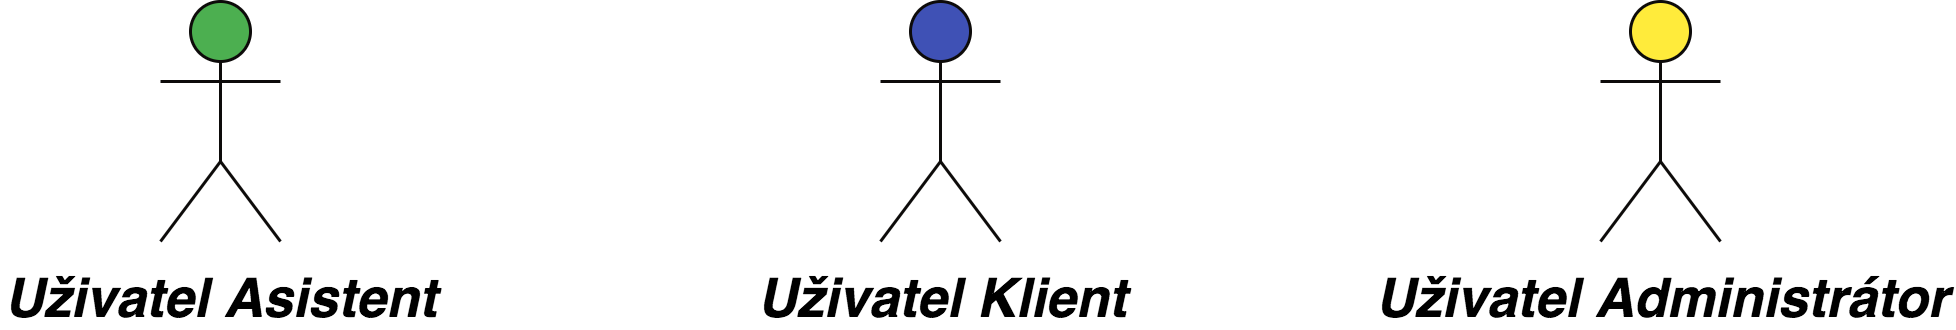
\includegraphics[scale=0.15]{img/actors.png}
        \caption{Aktéři systému}
        \label{fig:actors}
\end{figure}

\subsubsection{Uživatel Asistent}
Jedná se o aktéra, který je zároveň klientovi s mentálním postižením odborným asistentem,
jenž o něj pečuje a poskytuje mu podporu. Tento aktér je releventní k vytváření obsahu,
který má pomoci klientovi k lepší orientaci při cestování a také mu může připravenou
cestu předvést. Může také nahraná data editovat a případně je rozšiřovat. Může také zadat
do aplikace zadat své kontaktní údaje pro možnou nečekanou situaci klienta na cestách, případně
nastavit zálohování uložených dat pro zamezení jejich ztráty při ztrátě telefonu nebo jeho výměně
za jiný.

\subsubsection{Uživatel Klient}
Klient je osoba pro kterou je aplikace primárně určena a má mu pomoci vyřešit problém,
v tomto případě pomoci z orientací při cestování. Může si prohlížet obsah a zejména ho
využívat při cestách v terénu. Uživatel by měl být upozorněn na všechny uložené a rozeznané
data v závisloti na své pozici a měl by tak získat releventní informace k tomu, kde se právě
nachází. Dále může aplikaci využít ke snadnému kontaktování svého asistenta.

\subsubsection{Uživatel Administrátor}

\subsection{Use casy}
Pro uživatele klienta i asistenta jsou definovány případy užití zvlášť, neboť se celé chodvání
a použití aplikace bude v obou případech značně lišit.

\subsubsection{Uživatel asistent}
Pro uživatele asistnta jsou určeny složitější operace pro vytváření interaktivního obsahu pro klienta,
nastavování aplikace a prezentace klientovi. Pro use casy asistenta platí, že klient může těmto
krokům přihlížet, pokud o to projeví zájem.

\begin{figure}[H]
        \centering
                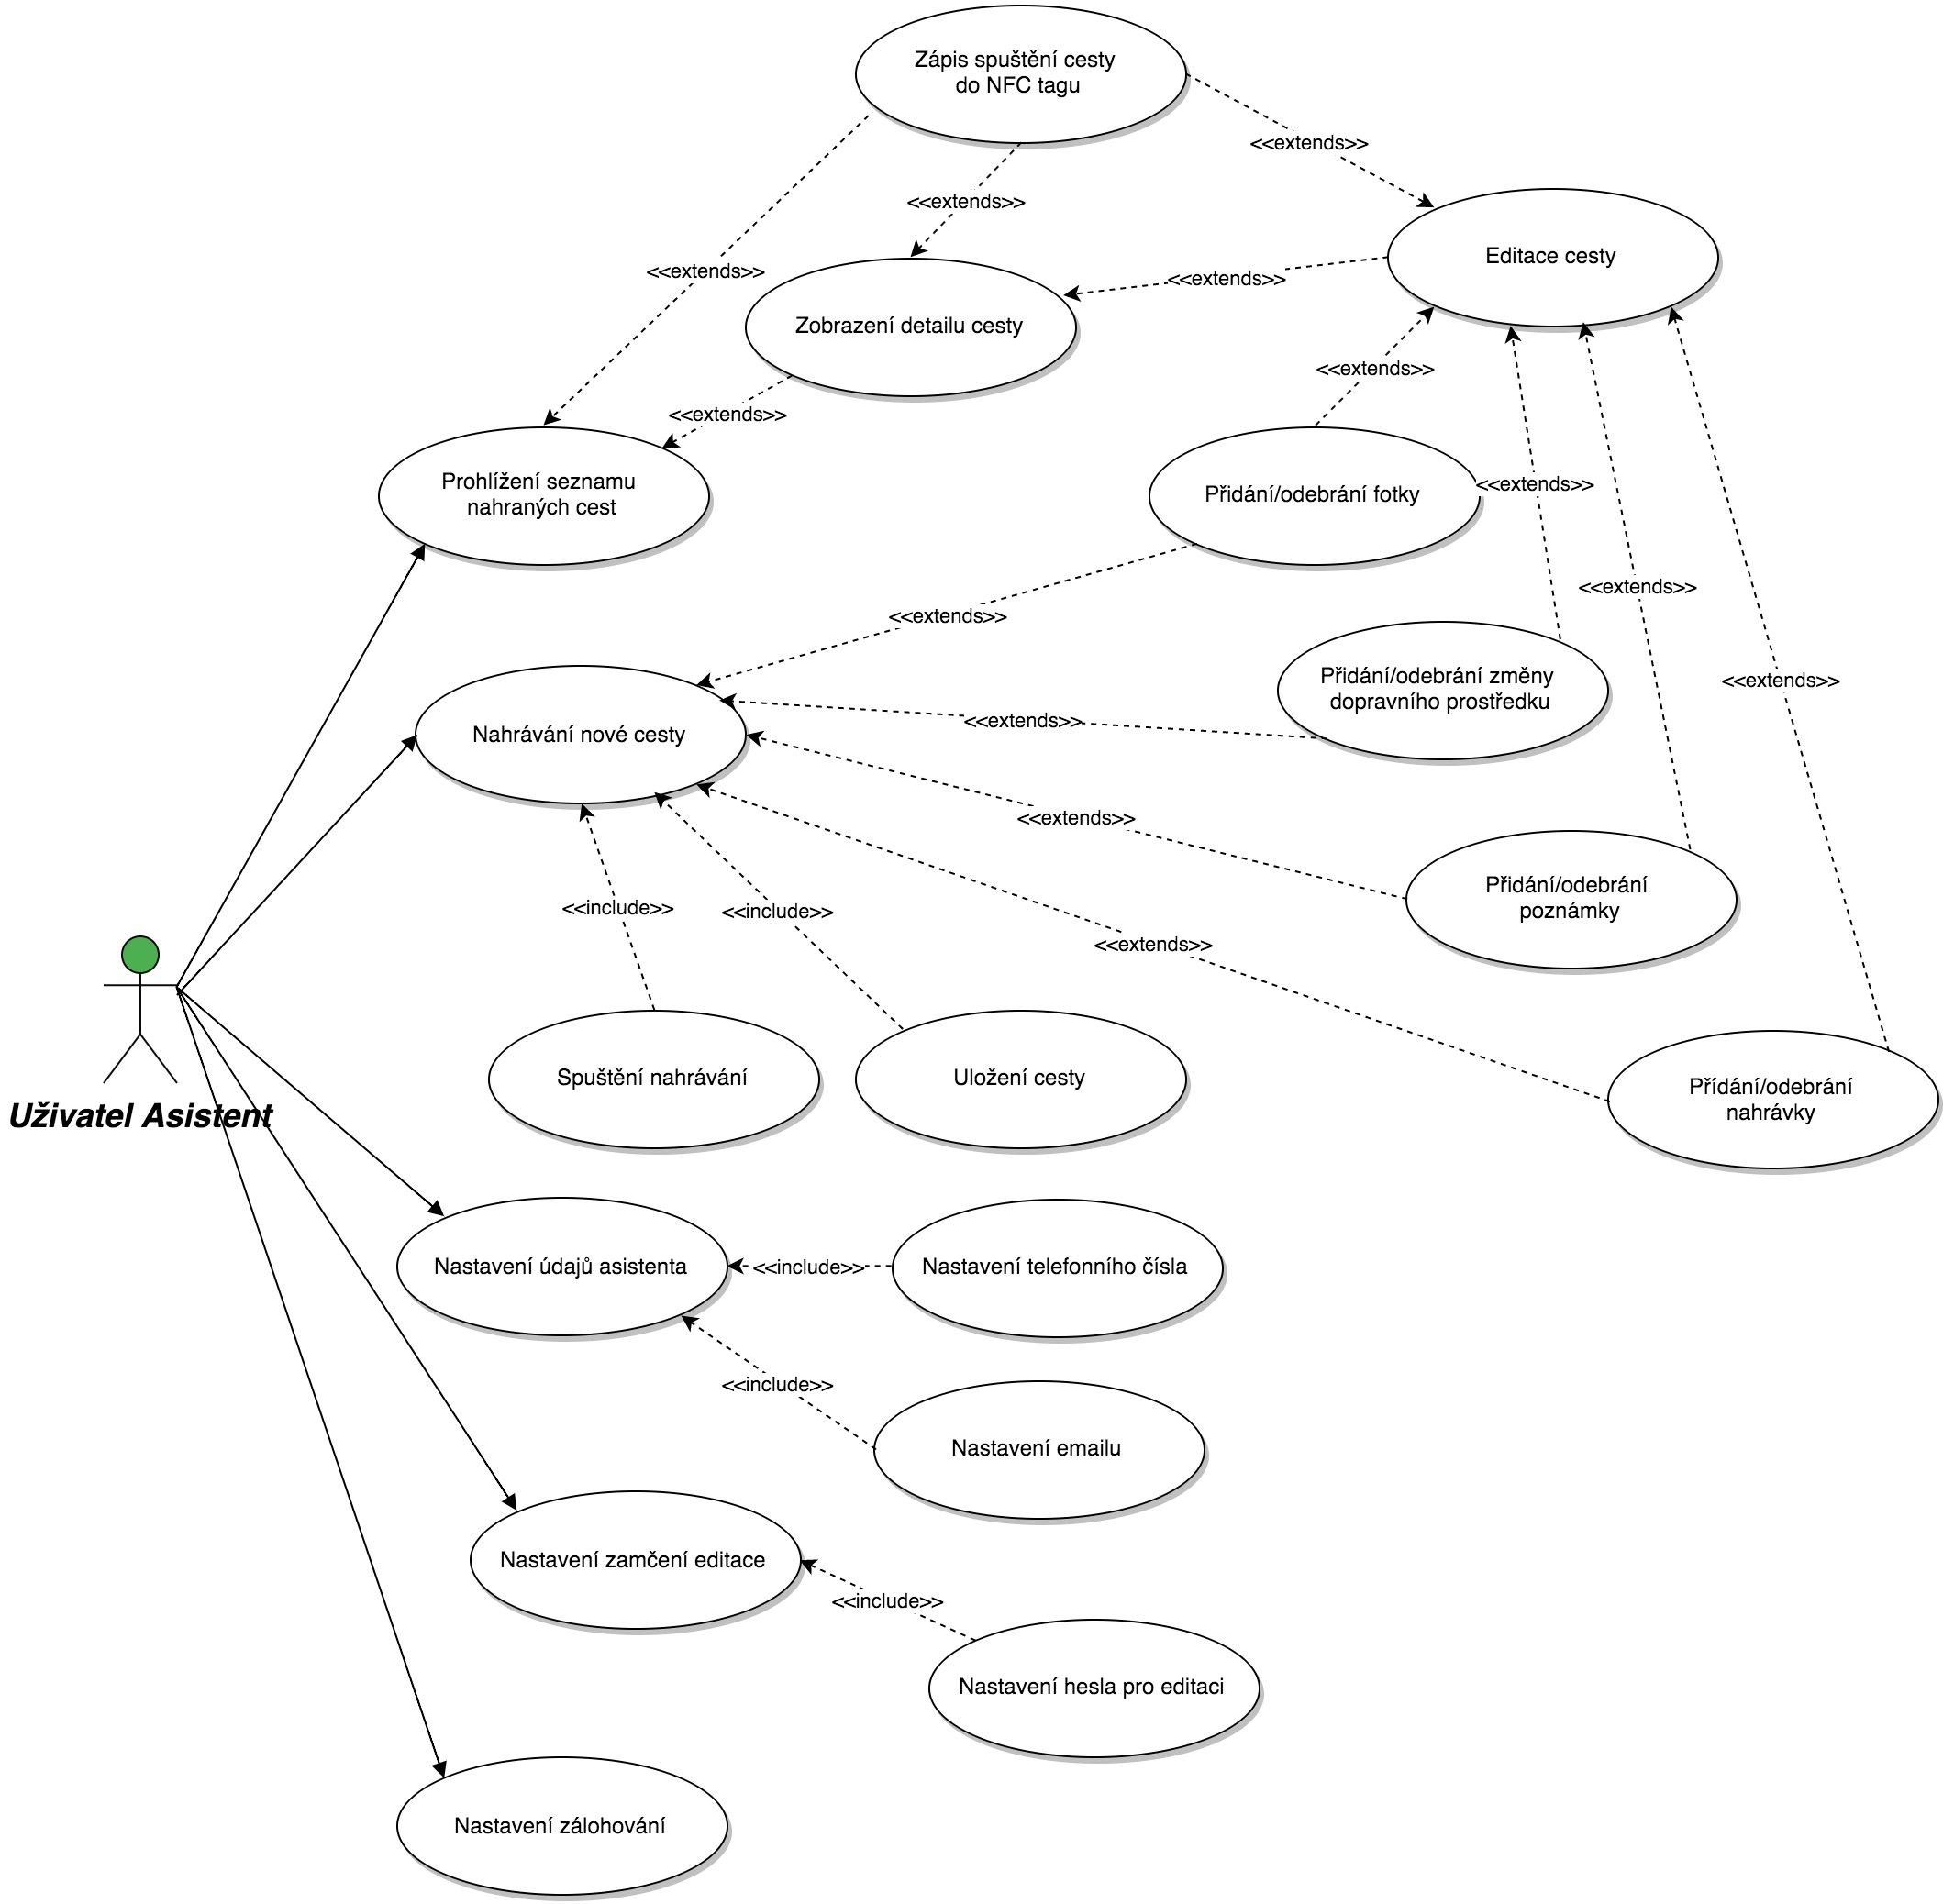
\includegraphics[scale=0.2]{img/UseCasesAsistant.png}
        \caption{Diagram use casů uživatele asistent}
        \label{fig:UseCasesAsistant}
\end{figure}

%\usecase{name}
%\textbf{Aktéři:} Asisitent
%
%\vspace{0.1cm}
%\noindent
%\textbf{Hlavní scénář:}
%
%\vspace{0.1cm}
%\noindent
%\textbf{Prekondice:}
%
%\vspace{0.1cm}
%\noindent
%\textbf{Spouštěč:}
%
%\vspace{0.1cm}
%\noindent
%\textbf{Rozšíření:}



\subsubsection{Uživatel klient}
Pro klienta jsou určeny více intuitivní a nenáročné operace vyžadující co nejméně aktivních
kroků z klientovi strany. Aplikace by měla na základě polohy a dalších údajů sama rozpoznat,
co má v  danou chvíli udělat.

\begin{figure}[H]
        \centering
                \includegraphics[scale=0.2]{img/UseCasesClient.png}
        \caption{Diagram use casů uživatele klient}
        \label{fig:UseCasesClient}
\end{figure}



\subsection{Použité nástroje}
\subsubsection{draw.io (\url{http://www.draw.io})}
Online nástroj pro tvorbu grafů, všech různých typů diagramů, myšlenkových map a dalších.
Celý edior běží pouze v prohlížeči a synchronizuje vytvářené grafy s připojeným úložištěm
Google Drive nebo Dropbox. Grafy jsou tak přístupné  a editovatelné odkudkoliv a aplikace
je opravdu pokročilá a při práci není vůbec poznat, že vše probíhá pouze v prohížeči.
Umožňuje sdílení i export zhotovených diagramů do mnoha formátů a je tedy velice snadné
sdílet a používat vytvořenou práci.
Nástroj byl použit pro vytváření use case diagramů a třídnách diagramů v této práci.
\begin{figure}[H]
        \centering
                
\includegraphics[scale=0.2]{img/drawiologo.png}
        \caption{Logo nástroje draw.io}
        \label{fig:iologo}
        \centering Zdroj: \url{http://www.draw.io}
\end{figure}

%\subsection{Podnadpis\footnote{Inspirace v \cite{saad}}}



\section{Závěr}


\begin{thebibliography}{99}

\end{thebibliography}

  \appendix

  \section{Zdrojové kódy}
  Kódy lze nalézt i na přiloženém CD.

\end{document}